\chapter{Introduction}\label{ch:intro}

In this chapter we are going to describe accurately the problem and provide a possible 
solution (from the point of view of a Distributed Systems designer).\\


\section{The Problem}

The bridge has:
\begin{itemize} 
    \item \textbf{maximum capacity} $c \geq 1$ 
    \item \textbf{length} $l \geq 1$
\end{itemize}

Cars can send messages to adjacent cars (to the car in front and to the rear one); 
cars can also have the ability to speak with more than two other cars depending on the 
\textbf{power of their transmission medium} $p \geq 1$.\\

So basically a car can only send messages to the $p$ cars in front and 
to the $p$ cars behind. We assume that the bridge length doesn't constitute an impediment 
for the communications (so even if the bridge was very long, however, 
the cars can send messages as if they were close).\\

Moreover a car has a certain \textbf{speed} $s \geq 1 \frac{block}{s}$ that determines 
the bridge crossing time and the time to reach the first obstacle 
(another enqueued car or the bridge).\\ 

For simplicity we assume that every car has the 
same dimensions expressed in an arbitrary length scale called \textbf{block} and 
\textbf{every measure is an integer} ($s$, $l$, $c$, $p$, etc.). \\

\begin{figure}
    \centering
    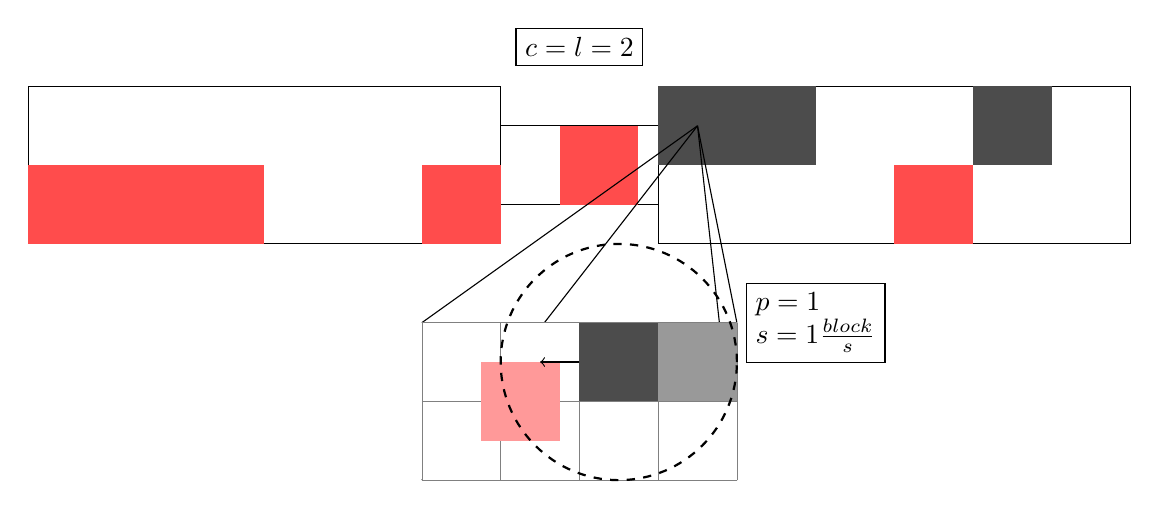
\begin{tikzpicture}
        % queues
        \draw (1,-1) rectangle (7,1);
        \draw (-7,-1) rectangle (-1,1);
        
        % bridge
        \draw (-1,-0.5) rectangle (1,0.5);
        \fill[red!70!white] (-0.25,-0.5) rectangle (0.75,0.5);
        \fill[red!70!white] (4,-1) rectangle (5,0);
        \node[draw,align=left] at (0,1.5) {$c = l = 2$};
        
        % left cars
        \fill[red!70!white] (-7,-1) rectangle (-6,0);
        \fill[red!70!white] (-6,-1) rectangle (-5,0);
        \fill[red!70!white] (-5,-1) rectangle (-4,0);
        \fill[red!70!white] (-2,-1) rectangle (-1,0);
        
        %% right cars
        \fill[black!70!white] (1,0) rectangle (2,1);
        \fill[black!70!white] (2,0) rectangle (3,1);
        \fill[black!70!white] (5,0) rectangle (6,1);
        
        \draw[black] (1.5,0.5) -- (-2, -2);
        \draw[black] (1.5,0.5) -- (2, -2);
        \draw[black] (1.5,0.5) -- (-2, -4);
        \draw[black] (1.5,0.5) -- (2, -4);

        % grid
        \fill[white]  (-2,-4) rectangle (2, -2);
        \draw[step=1cm,gray,very thin] (-2,-4) grid (2, -2);
        \fill[black!70!white] (0,-3) rectangle (1,-2);
        \fill[black!40!white] (1,-3) rectangle (2,-2);
        \fill[red!40!white] (-1.25,-3.5) rectangle (-0.25,-2.5);

        \draw[black,thick,dashed] (0.5,-2.5) circle (1.5cm);
        \node[draw,align=left] at (3,-2) {$p = 1$\\ $s = 1 \frac{block}{s}$};
        \draw[->,black] (0,-2.5) -- (-0.5, -2.5);
    \end{tikzpicture}
    \caption{Example of a possible situation} \label{fig:1}
\end{figure}
